%!TEX root = ../main.tex

%!TEX root = ../main.tex

\chapter{Reinventing Gillian's Logging Structure}\label{sec:log-structure}
\todo{Write section}

%!TEX root = ../main.tex

\chapter{Reconfiguring the Interpreter for Branched Execution}\label{sec:branched-exec}
\todo{Write section}

%!TEX root = ../main.tex

\section{A Rich Debugging Interface}\label{sec:debug-interface}
\todo{Write section}


\chapter{Debugger Improvements}\label{sec:improvements}
\todo{Trash / reincorporate into other sections}

\section{Debugging Unification}\label{sec:improvements:unification_debug}

\subsection{Log Report Structure}\label{sec:improvements:unification_debug:log_structure}

Before this project, the structure of reports from a Gillian verification
(\autoref{fig:log-structure-current}) were designed to accompany a linear
debugging presentation, going line-by-line in the source file, and not
considering any details concerning unification. Note that this figure has
assertion reports, which weren't present before this project; they were placed
as-is into the original logging structure at the start of the project.

After careful consideration, and correspondance with existing Gillian
developers, the plan for an improved logging structure formed
(\autoref{fig:log-structure-desired}). This new structure is built around the
prospect of users navigating through the verification process in a tree-of-trees
structure, not dissimilar from how Gillian processes this verification
internally. Of particular significance is the deliberate placement of
`previous-next' and `parent-child' connections between reports to signify
`the next step' and `more detail on the current step' respectively.

The main advantage of the latter structure is how each section of execution /
unification is inherently representive of how one would understand the
verification process, whereas the former requires additional annotation for
such information to be apparent.

In terms of actual implementation, Gillian's underlying reporting infrastructure
was already fit-for-purpose, with the inclusion of optional `parent' and
`previous' references for each report; the code only required some modification
to allow a greater degree of control over these properties in order to build a
more involved logging structure.

\newgeometry{top=0.5cm,bottom=2cm,left=1cm,right=1cm}

\begin{sidewaysfigure}
  \center{}
  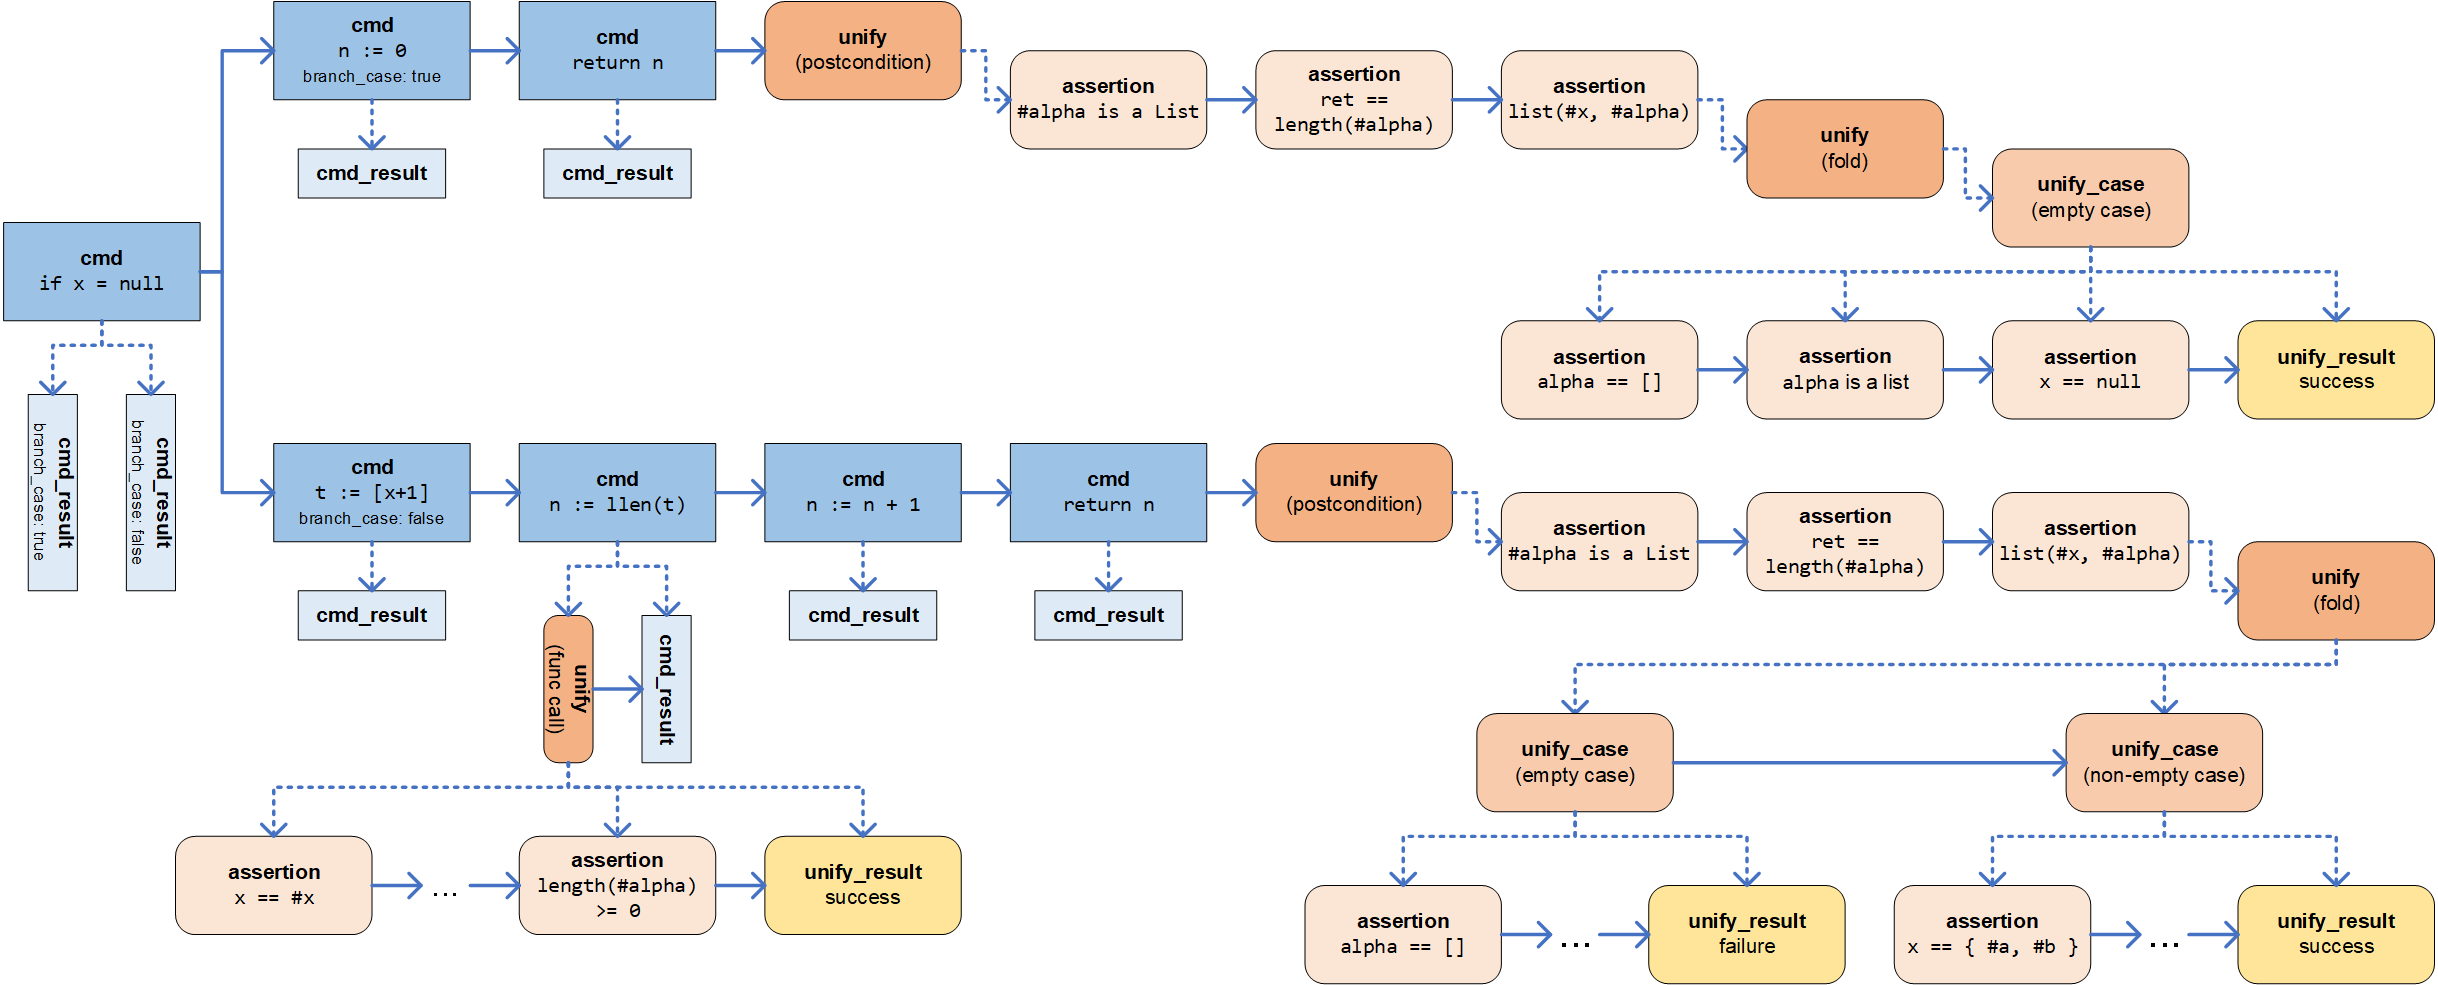
\includegraphics[width=0.95\textwidth]{img/log-structure-desired.png}
  \caption{The planned reporting structure for Gillian debugging}\label{fig:log-structure-desired}
\end{sidewaysfigure}

\restoregeometry{}
